\chapter{Аналитическая часть}

Для данной лабораторной работы, которая предполагает конвейерную обработку,
были выбраны три алгоритма для трех лент конвейера:

\begin{enumerate}
	\item Найти max в массиве;
	\item Найти min в массиве;
	\item Найти количество элементов в массиве, которые больше,
	      чем (max - min) / 2.
\end{enumerate}

\section{Описание метода}

\textit{Конвейер} - устройство для непрерывного перемещения обрабатываемого
изделия от одного рабочего к другому или для транспортировки грузов.

\textit{Конвейерное производство} - система поточной организации производства на основе конвейера,
при которой оно разделено на простейшие короткие операции, а перемещение деталей осуществляется автоматически.

В данной лабораторной работе мы выделяем три задачи, которые будут
последовательно обрабатываться на конвейерной ленте. Каждая задача
будет последовательно проходить три этапа обработки. Благодаря
распараллеливанию мы сможем добиться того, что бы на всех трех
этапах происходила обработка элемента, как в реальной жизни.

На рис \ref{ref:img1} визуализирован конвейер.

\begin{figure}[ht!]
	\centering{
		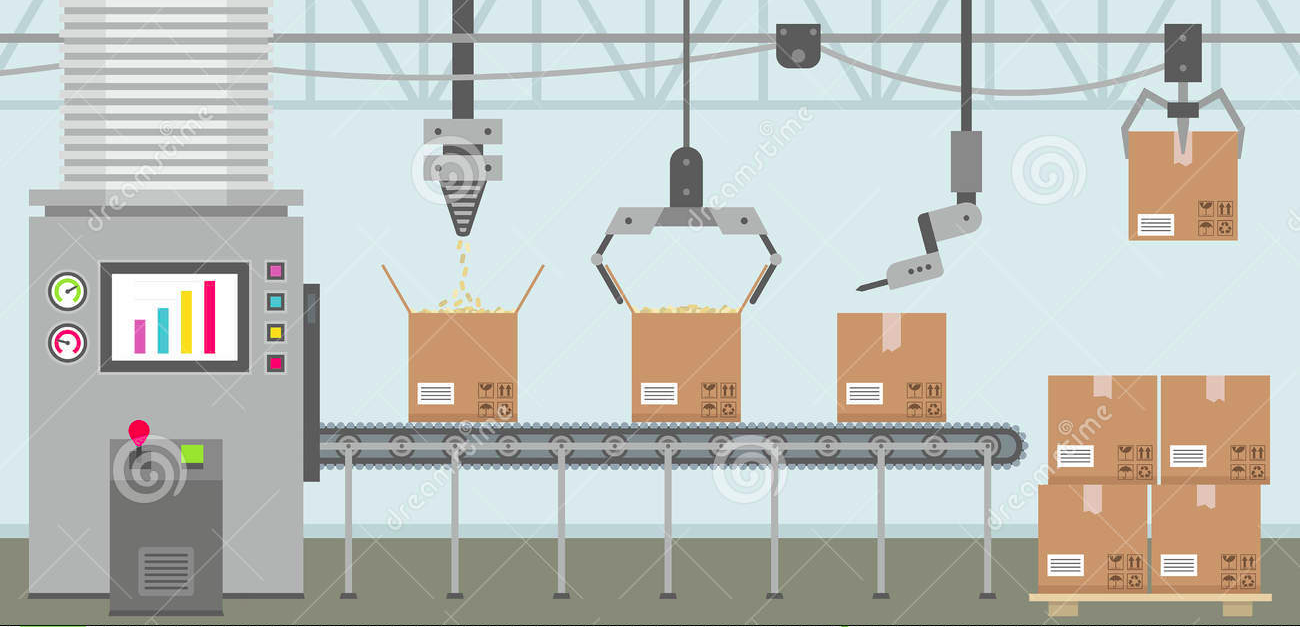
\includegraphics[width=0.9\textwidth]{conveyor_example.png}
		\caption{Конвейер}
		\label{ref:img1}}
\end{figure}


\section{Вывод}

В данном разделе были рассмотрены
основополагающие материалы, которые в дальнейшем потребуются
при реализации конвейера.
